\documentclass[../../main.tex]{subfiles}
 
\begin{document}

\section{Лекция 5. 20 ноября 2019 г.}
\vspace{10pt}

\vspace{10pt}

$X, Y$ — топологические пространства, $x \in X$

\defn отображение $f\colon X \rightarrow Y$ \textbf{непрерывно} в $x \lra \ex окр \; V \ni f(x) \ex окр \; U \ni x \colon f(U) \subset V$

$f$ \textbf{непрерывно}, если $f$ непрерывно в $x \; \fo x \in X$

\textbf{Теорема.} Следующие утверждения эквивалентны:

(1) $f$ непрерывно,

(2) $\fo окрестности \; V \subset Y \;\; f^{-1}(V)$ открыто в $X$,

(3) $\fo$ замкнутого $B \subset Y f^{-1}(B)$ замкнуто в $X$,

(4) $\fo A \subset X \;\; f(\overline{A}) \subset \overline{f(A)}$

\textit{Доказательство:}

$(1) \Ra (2)$ Пусть $V \subset Y$ — открыто.

$\fo x \in f^{-1}(V) \ex$ окр $U_x \ni x \colon f(U_x) \subset V \Ra U_x \subset f^{-1}(V) \Ra \bigcup_{x \in f^{-1}(V)} U_x = f^{-1}(V) \Ra f^{-1}(V)$ открыто.

$(2) \Ra (3)$ — следует из равенства $f^{-1}\left(Y \backslash B \right) = X \backslash f^{-1}(B) \quad \fo B \subset Y$

$(3) \Ra (4)$ $\fo A \subset X \quad A \subset f^{-1}\left( f(A) \right) \subset \underbrace{f^{-1}\left( \overline{f(A)} \right)}_{замкнуто} \Ra \overline{A} \subset f^{-1}\left( \overline{f(A)} \right), т.е. f(\overline{A}) \subset \overline{f(A)}$

$(4) \Ra (3)$ Пусть $B \subset Y$ замнкуто, $A = f^{-1}(B)$

$$f(\overline{A}) \subset \overline{f(A)} \subset \overline{B} = B \Ra \overline{A} \subset f^{-1}(B) = A, т.е. \; A \; замкнуто$$

Заметим, что $(2)$ и $(3)$ эквивалентны.

$(2) \Ra (1)$ $\fo x \in X$ пусть $V$ — окрестность $f(x) \Ra V = f^{-1}\left(V \right)$ — окрестность $x$, и $f(U) \subset V \quad \square$.

\textit{Следствие.} Пусть $\tau_1, \tau_2$ — топологии на множестве $X$. 

Тогда $\tau_1 \subset \tau_2 \lra $ отображение $f \colon \left(X, \tau_2 \right) \Rightarrow \left(X, \tau_1 \right),\; f(x) = x,$ непрерывно.

\textit{Предложение.} Пусть $f \colon X \to Y$ — отображение топологических пространств, $\sigma$ — предбаза $Y$.

$f$ непрерывно $\lra \fo V \in \sigma \;\; f^{-1}(V)$ открыто в $X$

\textbf{Доказательство: } $(\Leftarrow)$ Пусть $V \subset Y$ открыто $\Ra \; V = \bigcup_{\alpha \in A} \bigcap_{\beta \in B_{\alpha}} V_{\alpha\beta}$, где $V_{\alpha\beta} \in \sigma \Ra$

$\Ra f^{-1}(V) = \bigcup\limits_{\alpha \in A} \bigcap_{\beta \in B_{\alpha}} f^{-1}\left(V_{\alpha\beta} \right)$ — открыто в $X \quad \square$.

\textbf{Предложение.} $X, Y, Z$ — топологические пространства, $f \colon X \rightarrow Y, g\colon Y \Ra Z, \;\; x \in X,\; y = f(x)$

Предположение: $f$ непрерывно в $x, g$ непрерывно в $y \Ra g \circ f$ непрерывно в $x$.

В частности: если $f$ и $g$ непрерывны, то и $g \circ f$ непрерывно.

\begin{minipage}{0.5\linewidth}
\textit{Доказательство:} 

Пусть $W$ — окрестность $(g \circ f)(x) = g(x)$

$\left. 
\begin{gathered} 
\ex окрестность \; V \ni y \colon g(V) \subset W \\
\ex окрестность \; U \ni y \colon f(U) \subset V
\end{gathered}  
\right\}  \Ra (g \circ f)(U) \subset W$
\end{minipage}
\hfill
\begin{minipage}{0.5\linewidth}
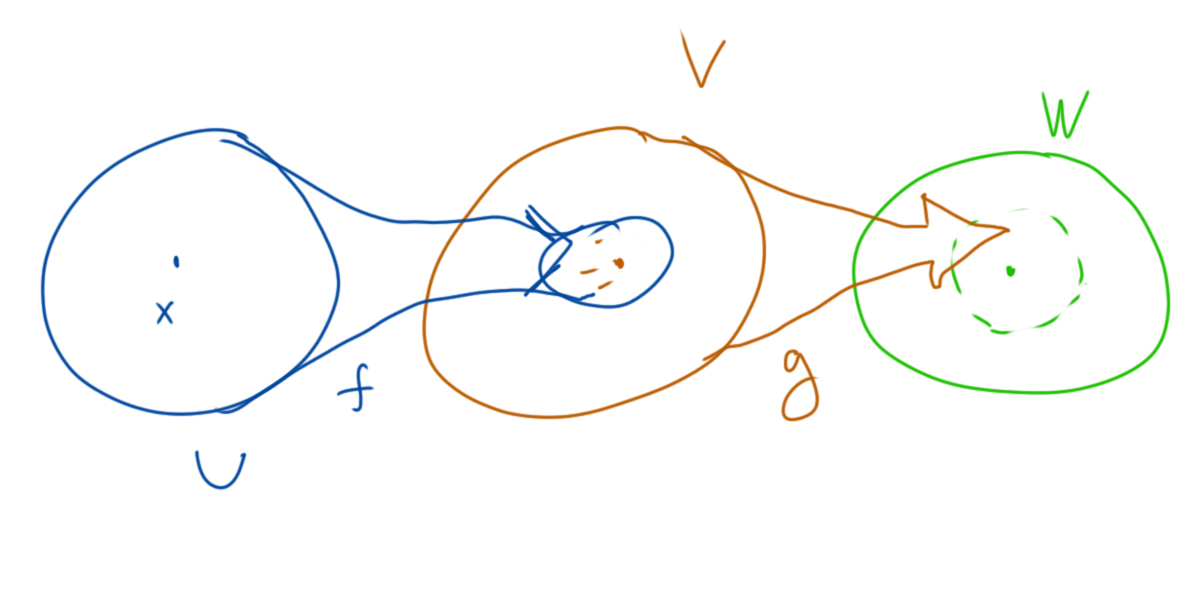
\includegraphics[width=7cm]{pictures/1.jpg}
\end{minipage}




\defn $X, Y$ — топологические пространства, $x \in X, f\colon X \to Y$

$f$ \textit{секвенциально непрерывно} в $x \lra \fo$ последовательности $(x_n)$ в $X$, т.ч. $x_n \to x$, выполнено $f(x_n) \to f(x)$.

\textbf{Предложение.} $f \colon X \to Y$ — отображение топологических пространств, $x \in X$.

(1) $f$ непрерывно в $x \Ra f$ секвенциально непрерывно в $x$.

(2) Если $X$ удовлетворяет 1-ой аксиоме счетности (непрерывно, метризуемо), то верно и обратное

\textit{Доказательство:} (1) Пусть $x_n \to x, \; V$ — окрестность $f(x)$

$\ex $ окрестность $U \ni x \colon f(U) \subset V$

$\ex N \in \N \; \fo n \geq N x_n \in U \Ra \fo n \geq N \;\; f(x_n) \in V \Ra f(x_n) \to f(x)$

(2) Предположение: $f$ не является непрерывным в $x$

$\ex$ база окрестностей $\left\{ U_n \colon n \in \N \right\}$ точки $x \colon U_n \supset U_{n+1}\;\; \fo n$

$\ex$ окрестность $V \ni f(x) \colon f(U_n) \not\subset V \;\; \fo n \in \N$

то есть $\fo n \in \N \; \ex x_n \in U_n, f(x_n) \notin V \Ra x_n \to x$, но $f(x_n) \not\to f(x)$ — противоречие. $\square$.

\textit{Обозначение.} $C(X, Y) = \left\{f \colon X \rightarrow Y \;|\; f \; непрерывно \right\}$

$C(X) = C(X, \K)$, где $\K = \R$ или $\mathbb{C}$.

\defn $f \in C(X, Y)$ — \textit{\textbf{гомеоморфизм}} $\lra \ex g \in C(Y, X) \colon fg = \id_{Y}$ и $gf = \id_X$

\defn\textbf{'} (эквивалентное предыдущему)

$f \colon X \to Y $ — \textit{\textbf{гомеоморфизм}} $\lra f$ непрерывно, биективно, и $f^{-1}$ непрерывно.

\textit{Наблюдение:} 

(1) $f\colon X \to Y, g\colon Y \to Z$ — гомеоморфизмы $\Ra g \circ f \colon X \to Z$ — гомеоморфизм.

\defn $X$ и $Y$ \textit{гомеоморфны} $\lra \ex$ гомеоморфизм $X \to Y$.

\defn $X, Y$ — топологические пространства, $f\colon X \to Y$.

$f$ \textit{открыто} $\lra \fo$ открытого $U \subset X \quad f(U)$ открыто в $Y$

$f$ \textit{замкнуто} $\lra \fo$ замкнутого $B \subset X \quad f(B)$ замкнуто в $Y$

\textit{Наблюдение:} 

Отображение $f\colon X \to Y$ — гомеоморфизм $\lra f$ непрерывно, биективно и открыто.

Отображение $f\colon X \to Y$ — гомеоморфизм $\lra f$   непрерывно, биективно и замкнуто.

\textbf{Пример-упражнение 1}. $X$ — нормированное пространство, $x \in X, r > 0$

$f \colon B_1(0) \to B_r(x), \quad f(y) = x + ry$ — гомеоморфизм.

\textbf{Пример-упражнение 2}. $X$ — нормированное пространство, $x \in X, r > 0$

$f \colon B_1(0) \to X,\; f(x) = \frac{x}{1 - ||x||}$ — гомеоморфизм.

\textbf{Пример-упражнение 3}. 

\begin{minipage}{0.6\linewidth}
$S^1 = \left\{ (x,y) \in \R \colon x^2 + y^2 = 1 \right\}$

$C = \left\{ (x, y) \in R \colon \max\left\{ |x|, |y| \right\} = 1 \right\}$

$f \colon C \to S^1, \quad f(p) = \frac{p}{||p||_2}$ — гомеоморфизм.
\end{minipage}
\hfill
\begin{minipage}{0.4\linewidth}
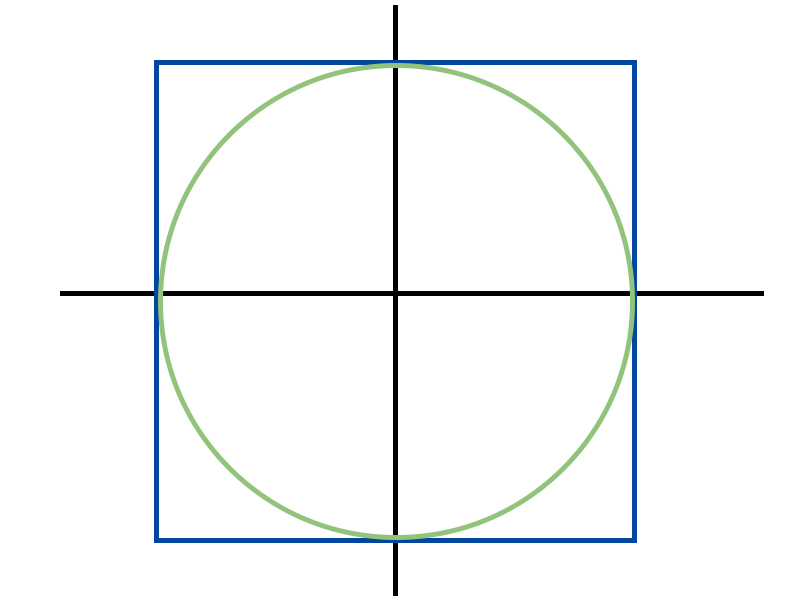
\includegraphics[width=7cm]{pictures/2.jpg}
\end{minipage}

\textbf{Пример-упражнение 4}. (стереографическая проекция)

(картинка 3)

$$S^2 = \left\{ (x,y) \in \R^3 \colon x^2 + y^2 + z^2 = 1 \right\} $$ — сфера

$f \colon S^2 \backslash\{N\} \to \R^2$ — гомеоморфизм


Построить аналогичный гомеоморфизм между $S^n \backslash \{N\}$ и $\R^n$

\defn Топологическое пространство $M$ — \textit{\textbf{топологическое многообразие}} ($C^0$-\textit{многообразие}) \textit{\textbf{размерности $n$}}, если

(1) $M$ хаусдорфово

(2) $M$ со счетной базой

(3) $\fo x \in X \; \ex $ окрестность $U \ni x$, гомеоморфная открытому подмножеству в $\R^n$ (здесь топология на $U$ определяется так: $V \subset U$ открыто в $U \lra V$ открыто в $M$)

Если $U$ — как в (3), $\varphi \colon U \to V$ — гомеоморфизм, где $V \subset \R^n$ открыто, то $(U, \varphi)$ называется \textit{картой} на $M$.

\textbf{Пример 1.} $\R^n$ — топологическое многообразие.

\textbf{Пример 2 - упражнение.} Открытое подмножество в $\R^n$ — топологическое многообразие (доказать наличие счетной базы)

\textbf{Пример 3 - упражнение.} Сфера $S^n \subset \R^{n+1}, S^n = \left\{x \in \R^{n+1} \colon ||x||_2 = 1 \right\}$ — топологическое многообразие.
Сколькими \textit{картами} она покрывается?

\subsection{Подпространства топологических пространств}

$(X, \tau)$ — топологическое пространство, $Y \subset X$

\textit{Обозначение.} $\tau_Y = \left\{ U \cap Y\; \colon \; U \in \tau \right\}$

\textit{Наблюдение.} $\tau_Y$ — топология на $Y$

\defn $\tau_Y$ — топология, \textit{индуцированная} (\textit{унаследованная}) из $(X, \tau)$.

\defn $(Y, \tau_Y)$ — называется \textit{топологическим подпространством} в $(X, \tau)$.

\textit{Предложение.} Пусть $(X, \ro)$ — метрическое пространство, $Y \subset X, \tau_{\ro}$ — топология на $Y$, порожденная ограничением метрики $\ro$ на $Y\times Y \; \Ra \tau_{\ro} = \tau_{Y}$.

\textit{Доказательство:} Базу $\tau_{\ro}$ образуют шары $B^Y_r(y) = \left\{ z \in Y \colon \ro(z,y) < r \right\} \quad \left(y \in Y, r > 0 \right)$

Заметим, что $B^Y_r(y) = B_r(y) \cap Y \quad$  (где $B_r(y) = \left\{ z \in X \colon \ro(z, y) < r \right\}) \Ra B^Y_r(y) \in \tau_Y \Ra \tau_{\ro} \subset \tau_Y$

Пусть $V \in \tau_{Y} \colon V = U \cap Y$, где $U$ открыто в $X$.

Пусть $y \in V \Ra \ex r > 0 \colon \; B_r(y) \subset U \Ra B^Y_r(y) \subset V \Ra V \in \tau_{\ro} \Ra \tau_Y = \tau_{\ro} \quad \square$.

(картинка 4). \textit{Обозначение}. $X$ — множество, $Y \subset X$

$i_Y \colon Y \to X, i_Y(y) = y \; \fo y \in Y$ — \textit{отображение включения} $Y$ в $X$.

\begin{theo}[(основное свойство индуцированной топологии)]{thm:ind_topology}

$(X, \tau)$ — топологическое пространство, $Y \subset X$. Снабдим $Y$ индуцированной топологией $\tau_Y$. Тогда:

(1) $\tau_Y$ — самая грубая\footnotemark{} топология на $X$ в которой $i_Y \colon Y \to X$ непрерывно,

(2) Если $Z$ — топологическое пространство, то $f \colon Z \to Y$ непрерывно $\lra i_Y \circ f \colon Z \to X$ непрерывно.

Иначе говоря: $f$ непрерывно как отображение из $Z$ в $Y \lra$ оно непрерывно как отображение из $Z$ в $X$.
\end{theo}\footnotetext{А существует ли самая тонкая? Да — дискретная.}

\textit{Доказательство:} 

(1) $i^{-1}_Y(U) = U \cap Y \Ra i_Y$ непрерывно.

Пусть $\sigma$ — топология на $Y$, т.ч. $i_Y \colon (Y, \sigma) \to X$ непрерывно $\lra \fo U \in \tau \;\; \underbrace{i^{-1}_Y(U)}_{= U \cap Y} \in \sigma \Ra \tau_Y \subset \sigma$.

(2) $\fo U \subset X$

$(i_Y\circ f)^{-1}(U) = f^{-1}\left( i^{-1}_Y(U) \right) = f^{-1}(U\cap Y)$

$i_Y\circ f$  непрерывно $\lra \fo U \in \tau (i_Y\circ f)^{-1}(U)$ открыто в $Z \lra \fo V \in \tau_Y \;\; f^{-1}(V)$ открыто в $Z \Ra f$ непрерывно $\square$.

\textit{Упражнение.} $\tau_Y$ — единственная топология на $Y$, удовл (1), и единственная топология на $Y$, удовлетворяющая (2).





\end{document}